\part{Magnetostatics}
    \section{The Magnetic Field}
    \subsection{The Magnetic Force}
    The \define{magnetic field}, \(\vv{B}\), is defined by the force, \(\vv{F}\), experienced by a charge, \(q\), with velocity \(\vv{v}\), in an external electric field \(\vv{E}\):
    \[\vv{F} = q(\vv{E} + \vv{v}\times\vv{B}).\]
    This is called the \define{Lorentz force law}.
    The units of \(\vv{B}\) are teslas, \si{\tesla}, defined by \(\SI{1}{\tesla} = \SI{1}{\newton.\ampere^{-1}.\metre^{-1}}\).
    This is quite a large unit and it is common to use an alternative unit called a gauss defined by \(\SI{e-4}{\tesla} = \SI{1}{\gauss}\) sometimes also denoted \(\SI{1}{\gaussAlternate}\).
    
    The important thing about this formula is that the force due to the magnetic field, \(\vv{v}\times\vv{B}\), is perpendicular to the velocity.
    This means that magnetic fields do no work as \(\vv{v}\cdot(\vv{v}\times\vv{B}) = \vv{0}\).
    
    \subsection{Current}
    A \define{current} is a moving density of charge.
    For a \define{steady current} at any point, \(\vv{r}\), a constant (time independent) density of charge moves past \(\vv{r}\) in a given time.
    Steady currents are important as if all currents are steady we will see that this leads to a constant magnetic field in the same way that stationary charges lead to a constant electric field.
    A current formed by \(n(\vv{r})\) charges, \(q\), moving past the point \(\vv{r}\) with average velocity \(\vv{v}(\vv{r})\) can be described by a \define{current density}
    \[\vv{J}(\vv{r}) = n(\vv{r})q\vv{v}(\vv{r}) = \rho(\vv{r})\vv{v}(\vv{r}).\]
    Here we have used \(n(\vv{r})q = \rho(\vv{r})\).
    The current density is to the magnetic field as the charge density is to the electric field.
    The units of \(\vv{J}\) are \(\si{\ampere.\metre^{-2}}\).
    We can similarly define a surface current density, usually denoted \(\vv{K}\) or \(\vv{j}\).
    This will have units of \(\si{\ampere.\metre^{-1}}\).
    We can also define a line current density, usually denoted \(\vv{I}\), which has units of \(\si{\ampere}\).
    
    The total current, \(I\), is the current density through a surface, \(A\):
    \[I = \int_A \vv{J}\cdot\dd{\vv{S}},\]
    where \(\dd{\vv{S}}\) is a surface element normal to \(A\).
    
    \begin{example}
        An insulating disc of radius \(R\) with uniform charge density, \(\sigma\), is rotated about its axis with an angular velocity, \(\vv{\omega} = \omega\ve{z}\).
        As a result the disc has a surface current density:
        \[\vv{K} = \sigma\vv{v} = \sigma\vv{\omega}\vv{r} = \sigma\omega\ve{z}\times r\ve{\rho} = \sigma\omega r\ve{\varphi}.\]
        Notice that this is a steady current even though the disc is moving faster towards the edge, hence scaling with \(r\).
        The important thing for a steady current is that the current is constant at any one point in space, not that it has the same value at all points of space.
    \end{example}
    
    \subsection{Conductivity}
    The \define{conductivity}, \(\sigma\), is an intrinsic bulk property of a material.
    It relates the current density to the electric field:
    \[\vv{J} = \sigma\vv{E}.\]
    This is \define{Ohm's law}.
    This assumes that \(\vv{J}\) and \(\vv{E}\) are parallel.
    This is only the case if the material is isotropic, that is all directions within the material are equivalent.
    If this isn't the case then we need to use the conductivity tensor, \(\sigma_{ij}\), instead.
    
    A typical value of \(\sigma\) for a metal is \(\SI{e9}{\ohm^{-1}.\metre^{-1}}\).
    We define the \define{resistivity} as
    \[\rho = \frac{1}{\sigma}.\]
    A typical value of \(\rho\) for an insulator is \(\SI{e16}{\ohm.\metre}\).
    In a superconductor \(\rho = 0\).
    
    Suppose a wire of cross sectional area \(A\) has a homogenous current density and electric field.
    The current in the wire is
    \[I = \int_A\vv{J}\cdot\dd{\vv{S}} = \int_A J\dd{S} = \int \sigma E\dd{S} = E\sigma A.\]
    The potential difference between two points on the wire a distance \(d\) apart is
    \[\Delta V = Ed.\]
    The current can then be written as
    \[I = \frac{A\sigma}{d}\Delta V.\]
    Rearranging we get
    \[\Delta V = IR,\qquad\text{where}\qquad R = \frac{d\rho}{A}.\]
    \(R\) here is what we define as the \define{resistance}.
    It has units of ohms, \(\si{\ohm}\).
    This equation is the more familiar form of Ohm's law.
    
    \subsection{Current Elements}
    A current element, \(\dd{\vv{\current}}\), is a vector defined by
    \begin{align*}
        \dd{\vv{\current}(\vv{r})} &= \vv{J}(\vv{r})\dd{V},\\
        \dd{\vv{\current}(\vv{r})} &= \vv{K}(\vv{r})\dd{S},\\
        \dd{\vv{\current}(\vv{r})} &= \vv{I}(\vv{r})\dd{l}.
    \end{align*}
    The units of a current element are \(\si{\ampere.\metre}\).
    Be careful, \(\vv{K}\dd{S} \ne K\dd{S}\), the first points in the direction of the surface current density, which is along the surface, and the second is normal to the surface.
    On the other hand \(\vv{I}\dd{l} = I\dd{\vv{l}}\) since a line current element always points along the line and so does a line element.

    A current is a moving charge element.
    For a bulk current density we have
    \[\dd{\vv{\current}}(\vv{r}) = \vv{J}(\vv{r})\dd{V} = \rho(\vv{r})\vv{v}(\vv{r})\dd{V} = \vv{v}(\vv{r})\dd{q}.\]
    This means that we can work out the force, \(\dd{\vv{F}}\), on a current element, \(\dd{\vv{\current}}\), in a magnetic field, \(\vv{B}\):
    \[\dd{\vv{F}} = \dd{q}\vv{v}\times\vv{B} = \dd{\vv{\current}}\times\vv{B}.\]
    If the current comes from a bulk current density, \(\dd{\vv{\current}} = \vv{J}\dd{V}\) then
    \[\dd{\vv{F}} = \vv{J}\times\vv{B}\dd{V}.\]
    
    \subsection{Biot Savart Law}
    The Biot Savart law is an empirical law relating current elements to the magnetic field.
    It states that if a current element \(\dd{\vv{\current}}(\vv{r'})\) is at position \(\vv{r'}\) then the resulting magnetic field at \(\vv{r}\) is given by
    \[\dd{\vv{B}(\vv{r})} = \frac{\mu_0}{4\pi} \frac{\dd{\vv{\current}(\vv{r'})} \times (\vv{r - \vv{r'}})}{\abs{\vv{r} - \vv{r'}}^3}.\]
    The Biot Savart law is to magnetic fields as Coulomb's law is to electric fields.
    It states that charge elements create magnetic fields which shows that a steady current causes a constant magnetic field.
    Here \(\mu_0\) is a constant known as the permeability of free space, or the electric constant.
    It has a value of
    \[\mu_0 = 4\pi\cdot\SI{e-7}{\henry.\metre^{-1}} = 4\pi\cdot\SI{e-7}{\newton.\ampere^{-2}}.\]
    Here \(\si{\henry}\) is a henry defined as \(\SI{1}{\henry} = \SI{1}{\newton.\metre.\ampere^{-2}}\).
    
    Since the Biot Savart law is linear in \(\dd{\vv{\current}}\) the superposition of the magnetic fields of many current elements to get the total magnetic fields holds so
    \[\vv{B}(\vv{r}) = \frac{\mu_0}{4\pi}\int \frac{\dd{\vv{\current}(\vv{r'})} \times (\vv{r} - \vv{r'})}{\abs{\vv{r} - \vv{r'}}^3}.\]
    For a bulk current density this becomes
    \[\vv{B}(\vv{r}) = \frac{\mu_0}{4\pi} \int \frac{\vv{J}(\vv{r'})\times(\vv{r} - \vv{r'})}{\abs{\vv{r} - \vv{r'}}^3} \dd[3]{r'}.\]
    
    \subsection{Magnetic Force Between Currents}
    The force on the current element \(\dd{\vv{\current_1}}\) at position \(\vv{r_1}\) due to a current element, \(\dd{\vv{\current_2}}\), at \(\vv{r_2}\) is
    \[\dd{\vv{F_1}} = \dd{\vv{\current_1}}\times\dd{\vv{B_2}} = \frac{\mu_0}{4\pi r_{12}^2} \dd{\vv{\current_1}} \times (\dd{\vv{\current_2}}\times \vhsub{r}{_{12}}).\]
    Here \(\dd{\vv{B_2}}\) is the magnetic field due to the second current element and \(\vv{r_{12}} = \vv{r_1} - \vv{r_2}\).
    If the each current element, \(\dd{\vv{\current_i}}\) is due to a bulk current density \(\vv{J_i}\) then this becomes
    \[\dd{\vv{F_1}} = \frac{\mu_0}{4\pi r_{12}^2} \vv{J_1}\times (\vv{J_2} \times \vhsub{r}{_{12}}) \dd[3]{r_1}\dd[3]{r_2}.\]
    
    \begin{example}
        A long straight wire is aligned along the \(z\)-axis.
        It carries a current, \(I\), in the positive \(z\) direction.
        What is the magnetic field strength at a point a distance \(r\) from the wire?
        
        A current element is given by
        \[\dd{\vv{\current}} = I\dd{z}\ve{z} = I\dd{\vv{r'}}\]
        where \(\vv{r'}\) is the position of the current element along the wire.
        Choosing the origin to be in the same plane as the point at which we are evaluating the field we have
        \[\vv{r} = \rho\ve{\rho}\]
        for the position at which we want to know the field strength (note that \(\rho\) here is cylindrical coordinates, not charge density or resistivity).
        Applying the Biot Savart law we get
        \begin{align*}
            \vv{B}(\vv{r}) &= \frac{\mu_0}{4\pi} \int \frac{\dd{\vv{\current}} \times (\vv{r} - \vv{r'})}{\abs{\vv{r} - \vv{r'}}^3}\\
            &= \frac{\mu_0}{4\pi} \int \frac{I\ve{z}\times(\rho\ve{\rho} - r'\ve{z})}{\abs{\vv{r} - \vv{r'}}^3} \dd{z}\\
            &= \frac{\mu_0}{4\pi} I \left[ \int \frac{\ve{z}\times\rho\ve{\rho}}{\abs{\vv{r} - \vv{r'}}^3} \dd{z} - \int \frac{\ve{z}\times r'\ve{z}}{\abs{\vv{r} - \vv{r'}}^3} \dd{z} \right]\\
            &= \frac{\mu_0 I}{4\pi}\rho\ve{\varphi}\int (\rho^2 + z^2)^{-3/2} \dd{z}\\
            &= \frac{\mu_0 I}{2\pi\rho}\ve{\varphi}.
        \end{align*}
        We looked up the integral in the last step over all \(z\in\reals\) and found it to be \(2/\rho^2\).
    \end{example}

    \section{Divergence and Curl of the Magnetic Field}
    \subsection{Divergence of the Magnetic Field}
    The Biot Savart law for a bulk current density, \(\vv{J}(\vv{r'})\), is
    \begin{align*}
        \vv{B}(\vv{r}) &= \frac{\mu_0}{4\pi} \int \vv{J}(\vv{r'}) \times \frac{(\vv{r} - \vv{r'})}{\abs{\vv{r} - \vv{r'}}^3} \dd[3]{r'}\\
        &= -\frac{\mu_0}{4\pi} \int \vv{J}(\vv{r'}) \times \grad_{\vv{r}}\left(\frac{1}{\abs{\vv{r} - \vv{r'}}}\right) \dd[3]{r'}
    \end{align*}
    Here we use a notation where differential operators with a subscript \(\vv{r}\) act only on the components of \(\vv{r}\).
    We can take the divergence of this fairly easily if we recognise that \(\vv{J}(\vv{r'})\) is constant with respect to \(\vv{r}\) so \(\grad_{\vv{r}}\cdot\vv{J}(\vv{r'}) = 0\).
    \begin{align*}
        \grad_{\vv{r}}\cdot\vv{B}(\vv{r}) &= -\frac{\mu_0}{4\pi} \int \grad_{\vv{r}}\cdot \left[\vv{J}(\vv{r'}) \times \grad_{\vv{r}}\left(\frac{1}{\abs{\vv{r} - \vv{r'}}}\right)\right] \dd[3]{r'}\\
        &= -\frac{\mu_0}{4\pi} \int \vv{J}(\vv{r'}) \cdot\left[\grad_{\vv{r}} \times \grad_{\vv{r}}\left(\frac{1}{\abs{\vv{r} - \vv{r'}}}\right)\right] \dd[3]{r'}\\
        &= 0
    \end{align*}
    Here we have used the identity that grad curl is zero.
    Hence
    \[\div\vv{B} = 0.\]
    This is \define{Maxwell's second law}.
    It states that there are no sinks or sources of the magnetic field,
    there are no magnetic monopoles, there are no point sources of the magnetic field, there are no `magnetic charges'.
    The magnetic field always forms closed loops.
    
    Applying the divergence theorem we have
    \[\int_V \div\vv{B}(\vv{r})\dd[3]{r} = \oint_A\vv{B}\cdot\dd{\vv{S}}.\]
    Identifying the left hand side as an integral of zero we have
    \[\oint_a\vv{B}\cdot\dd{\vv{S}} = 0.\]
    This is \define{Gauss' law for magnetic fields}.
    
    \subsection{Magnetic Dipoles}
    Maxwell's second law rules out the existence of magnetic monopoles.
    Therefore a magnetic dipole is the most elementary magnetic pole.
    It turns out that a magnetic dipole can be formed from a current loop.
    
    Suppose we have a circular loop or radius \(a\) carrying current \(I\).
    If we align the axis of the loop with the \(z\) axis so that the current is going in the \(\ve{\varphi}\) direction then the magnetic field on the axis can be found from the Biot Savart law,
    \[\dd{\vv{B}(\vv{r})} = \frac{\mu_0}{4\pi} \frac{\dd{\vv{\current}(\vv{r'})} (\vv{r} - \vv{r'})}{\abs{\vv{r} - \vv{r'}}^3}.\]
    Here \(\vv{r} = z\ve{z}\), \(\vv{r'} = a\ve{\rho}\), and \(\dd{\vv{\current}} = I\dd{\ell}\ve{\varphi}\).
    Hence
    \begin{align*}
        \dd{\vv{\current}} \times (\vv{r} - \vv{r'}) &= I\dd{\ell}\ve{\varphi} \times (z\ve{z} - a\ve{\rho})\\
        &= I\dd{\ell}(z\ve{\varphi}\times\ve{z} - a\ve{\varphi}\times\ve{\rho})\\
        &= I\dd{\ell}(z\ve{\rho} + a\ve{z}).
    \end{align*}
    Radial from diametrically opposed sides of the loop will cancel leaving a net field only in the \(\ve{z}\) direction:
    \[\dd{B_z} = \frac{\mu_0}{4\pi}\frac{Ia\dd{\ell}}{(a^2 + z^2)^{3/2}}\]
    Integrating this we get
    \begin{align*}
        B_z &= \frac{\mu_0}{4\pi} \frac{Ia}{(a^2 + z^2)^{3/2}} \oint\dd{\ell}\\
        &= \frac{\mu_0}{4\pi} \frac{Ia}{(a^2 + z^2)^{3/2}}2\pi a\\
        &= \frac{\mu_0Ia^2}{2(a^2 + z^2)^{3/2}}.
    \end{align*}
    At \(z = 0\) (i.e. the centre of the loop)
    \[B_z = \frac{\mu_0Ia^2}{2a^3} = \frac{\mu_0I}{2a}.\]
    In the far field (i.e. \(z \gg a\))
    \[B_z \approx \frac{\mu_0Ia^2}{2z^3}.\]
    It can be shown that off-axis field is
    \[\vv{B_{\mathrm{dip}}}(\vv{r}) = \frac{\mu_0}{4\pi r^3} [3(\vv{m}\cdot\vh{r})\vh{r} - \vv{m}]\]
    in the far field.
    Here \(\vv{m}\) is the dipole moment defined as
    \[\vv{m} = IA\ve{z}\]
    where \(A\) is the area of a current loop, in the \((x, y)\)-plane, and \(I\) is the current it carries.
    In this case \(A = \pi a^2\) so
    \[\vv{m} = I\pi a^2\ve{z}.\]
    More generally we can define the dipole moment as
    \[\vv{m} = I\vv{A} = I\int_A\dd{\vv{S}}\]
    where \(\vv{A}\) is the vector area of the loop defined by an integral over the entire loop, which may not be planar, and has surface elements \(\dd{\vv{S}}\).
    
    In an external magnetic field, \(\vv{B_\mathrm{ext}}\), a magnetic dipole has energy
    \[U = -\vv{m}\cdot\vv{B_\mathrm{ext}}.\]
    There is also a torque
    \[\vv{\tau} = \vv{m}\times\vv{B_\mathrm{ext}}.\]
    
    \subsection{Curl of the Magnetic Field}
    Starting again from the Biot Savart law for a bulk current density and this time taking the curl we have
    \[\grad_{\vv{r}} \times \vv{B}(\vv{r}) = -\frac{\mu_0}{4\pi} \int \grad_{\vv{r}} \times \left[\vv{J}(\vv{r'}) \times \grad_{\vv{r}}\left(\frac{1}{\abs{\vv{r} - \vv{r'}}}\right)\right] \dd[3]{r'}\]
    Looking just at the integrand we have
    \begin{align*}
        \grad_{\vv{r}} \times \left[\vv{J}(\vv{r'}) \times \grad_{\vv{r}}\left(\frac{1}{\abs{\vv{r} - \vv{r'}}}\right)\right] & = \vv{J}(\vv{r'})\laplacian_{\vv{r}}\left(\frac{1}{\abs{\vv{r} - \vv{r'}}}\right) - (\vv{J}(\vv{r'})\cdot\grad_{\vv{r}})\grad_{\vv{r}} \left(\frac{1}{\abs{\vv{r} - \vv{r'}}}\right)\\
        &= -4\pi\delta(\vv{r} - \vv{r'})\vv{J}(\vv{r'}) - (\vv{J}(\vv{r'})\cdot\grad_{\vv{r}}) \grad_{\vv{r}} \left(\frac{1}{\abs{\vv{r} - \vv{r'}}}\right).
    \end{align*}
    Hence the curl of the magnetic field is
    \begin{align*}
        \grad_{\vv{r}}\times\vv{B}(\vv{r}) &= \frac{\mu_0}{4\pi} \int 4\pi\delta(\vv{r} - \vv{r'})\vv{J}(\vv{r'}) \dd[3]{r'} + \frac{\mu_0}{4\pi} \int (\vv{J}(\vv{r'})\cdot\grad_{\vv{r}}) \grad_{\vv{r}} \left(\frac{1}{\abs{\vv{r} - \vv{r'}}}\right) \dd[3]{r'}
        \shortintertext{The second term can be shown to be zero by writing it as a boundary integral at infinity which must vanish to have finite energy}
        &= \frac{\mu_0}{4\pi} \int 4\pi\delta(\vv{r} - \vv{r'})\vv{J}(\vv{r'}) \dd[3]{r'}\\
        &= \mu_0\int \vv{J}(\vv{r'})\delta(\vv{r} - \vv{r'})\dd[3]{r'}\\
        &= \mu_0\vv{J}(\vv{r}).
    \end{align*}
    This is \define{Maxwell's fourth law}.
    Applying Stokes' theorem we have
    \[\int_S \curl\vv{B}\cdot\dd{\vv{S}} = \oint_C\vv{B}\cdot\dd{\vv{l}}.\]
    Looking at the left hand side we have
    \[\int_S \curl\vv{B}\cdot\dd{\vv{S}} = \mu_0 \int_S \curl\vv{J}\cdot\dd{\vv{S}} = \mu_0 I.\]
    Hence
    \[\oint_C\vv{B}\cdot\dd{\vv{l}} = \mu_0 I.\]
    This is \define{Ampere's law}.
    
    \begin{example}\label{exa:infinite wire magnetic field}
        Consider an infinite wire of radius \(a\) aligned along the \(\ve{z}\) direction carrying current density \(\vv{J}\propto\ve{z}\).
        We must have that \(B_z = 0\) as \(\vv{J}\) and \(\vv{B}\) must be perpendicular.
        Similarly we must have that \(B_\rho = 0\) as if there where radial components then \(\div\vv{B}\) would be non-zero violating the second of Maxwell's equations.
        Therefore \(\vv{B}\propto\ve{\varphi}\).
        Also \(B_\varphi\) cannot depend on \(z\) as we are free to place the origin anywhere along the wire and it cannot depend on \(\varphi\) as we are free to define any angle around the wire as \(\varphi = 0\).
        Thus we are left with
        \[\vv{B} = B_\varphi(\rho)\ve{\varphi}.\]
        For \(\rho > a\) we have
        \[\oint_C \vv{B}\cdot\dd{l} = B_\varphi 2\pi\rho = \mu_0 I_{\mathrm{enc}} = \mu_0 J\pi a^2.\]
        Hence
        \[B_\varphi = \frac{\mu_0 J}{2} \frac{a^2}{\rho}.\]
        For \(\rho < a\) we still have
        \[\oint_C \vv{B}\cdot\dd{\vv{l}} = B_\varphi 2\pi\rho\]
        but now
        \[\mu_0I_{\mathrm{enc}} = \mu_0J\pi\rho^2\]
        so
        \[B_\varphi = \frac{\mu_0J}{2}\rho.\]
        This is shown in figure~\ref{fig:magnetic field strength wire}.
        \begin{figure}[ht]
            \centering
            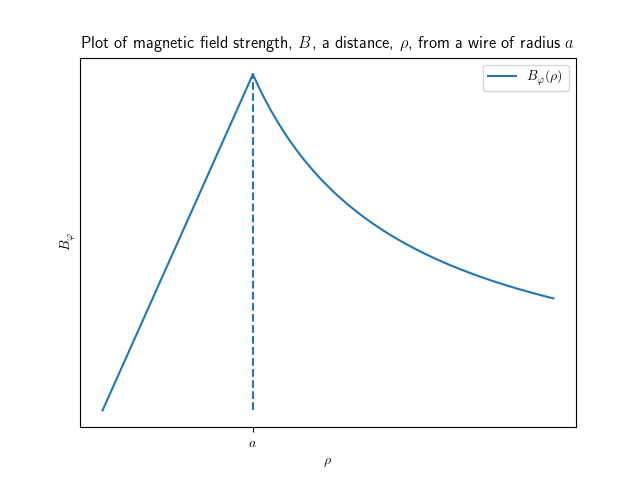
\includegraphics[scale=0.5]{magnetic_field_wire.png}
            \caption{The magnetic field strength a distance \(\rho\) from a wire.}
            \label{fig:magnetic field strength wire}
        \end{figure}
    \end{example}

    \section{Amp\`ere's Law and Vector Potentials}
    \subsection{Applications of Amp\`ere's Law}
    Amp\`ere's Law states
    \[\oint_C \vv{B}\cdot\dd{\vv{l}} = \mu_0 \int_A\vv{J}\cdot\dd{S} = \mu_0 I_\enc.\]
    Here \(\vv{B}\) is the magnetic field due to a current density \(\vv{J}\).
    \(C\) is some closed curve, called an Amp\`erian loop, bounding a surface \(A\) which has surface normals \(\dd{\vv{S}}\).
    \(I_\enc\) is the current that passes through the surface.
    The integration is performed along the curve in such a way that the surface normals and direction of integration agree with the right hand grip rule.
    Symmetry permitting Amp\`ere's law is usually the fastest way to calculate the magnetic field for a given current density.
    We look for cases where the Amp\`erian loop is either parallel or perpendicular to the magnetic field.
    The cases where this is possible and the Amp\`erian loops to use are
    \begin{itemize}
        \item Infinite straight line -- coaxial circles (see example~\ref{exa:infinite wire magnetic field})
        \item Infinite plane -- rectangular loop
        \item Infinite solenoid -- rectangular loop
        \item Toroid -- circle
    \end{itemize}
    \subsubsection{Infinite Slab of Current}
    An infinite slab of thickness \(d\) has a current density, \(\vv{J}\).
    Define the \(x\) direction to be the direction of this current density and the \(y\) direction to be in the slab but perpendicular to the current density and the \(z\) direction to be normal to the slab.
    
    The magnetic field cannot have an \(x\) component as the current density must be perpendicular to the magnetic field.
    The magnetic field cannot have a \(z\) component as if it did we could place a Gaussian surface with a section of the slab in it and the integral over it would be non-zero meaning that we would have non-vanishing divergence.
    This is forbidden by Maxwell's second law.
    This leaves us with a magnetic field that can only be in the \(y\) direction.
    
    If we choose to put the origin a distance \(d/2\) into the slab then since we can pick any point at this depth in the slab to place the origin we must have that \(B_y\) is independent of \(x\) and \(y\) and so \(B_y = B_y(z)\).
    
    We choose an Amp\`erian loop that is rectangular with two sides in the \(z\) direction and two in the \(y\) direction.
    The field is perpendicular to the sides in the \(z\) direction.
    The field is aligned with the sides in the \(y\) direction.
    Say that the length of these sides is \(b\), then
    \[\oint_C \vv{B}\cdot\dd{\vv{l}} = 2b\abs{B_y} = \mu_0I_\enc = \mu_0 bdJ\]
    \[\implies \abs{B_y} = \frac{1}{2}\mu_0 Jd.\]
    We know that \(\dd{\vv{\current}}\propto\ve{x}\) so for \(\vv{r}\propto\ve{z}\) we have, by the Biot Savart law, that
    \[\vv{B} \propto \vv{J}\times\vv{r} \propto \ve{x}\times\ve{z} = -\ve{y}\]
    This means that, outside of the slab, the magnetic field is
    \[
        \vv{B} =
        \begin{cases}
            -\frac{1}{2}\mu_0 Jd\ve{y}, & z > \frac{1}{2}d,\\
            +\frac{1}{2}\mu_0 Jd\ve{y}, & z < -\frac{1}{2}d.
        \end{cases}
    \]
    \begin{figure}[ht]
        \centering
        \tikzsetnextfilename{current-slab}
        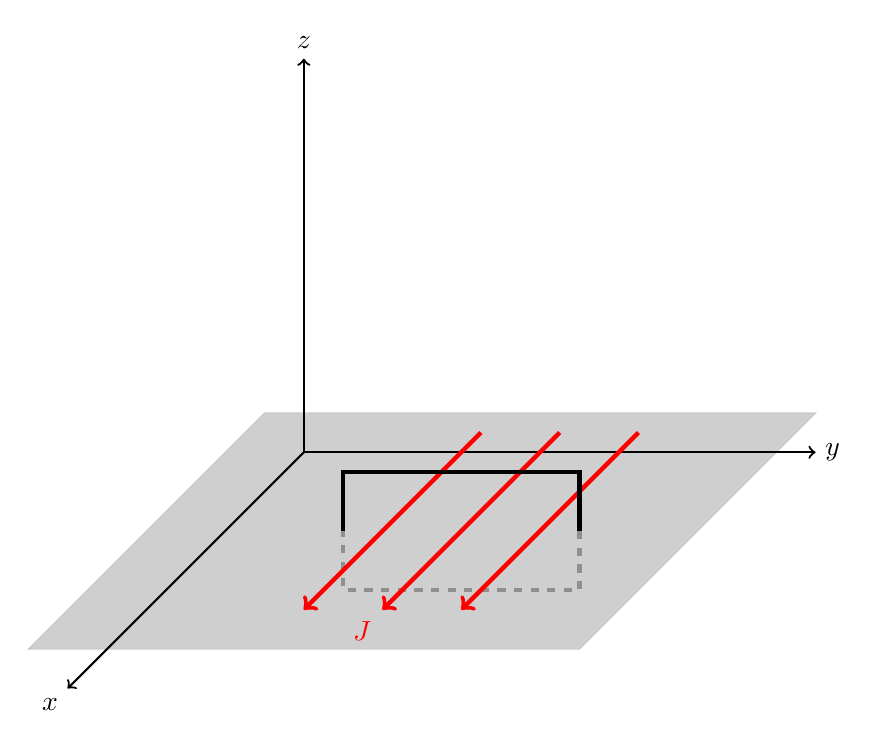
\begin{tikzpicture}
            \tikzstyle{current} = [color=red, ultra thick]
            \tikzstyle{axis} = [thick]
            \tikzstyle{conductor} = [color=lightgray, fill=lightgray, opacity=0.75]
            \tikzstyle{loop} = [ultra thick]
            \draw[dashed, loop] (3, -0.5) -- (3, -1.25) -- (0, -1.25) -- (0, -0.5);
            \draw[conductor] (-4, -2) -- (3, -2) -- (6, 1) -- (-1, 1) -- cycle;
            \begin{scope}[xshift=-0.5cm, yshift=0.5cm]
                \draw[axis, ->] (0, 0) -- (6.5, 0);
                \node[right] at (6.5, 0) {\(y\)};
                \draw[axis, ->] (0, 0) -- (0, 5);
                \node[above] at (0, 5) {\(z\)};
                \draw[axis, ->] (0, 0) -- (-3, -3);
                \node[below left] at (-3, -3) {\(x\)};
            \end{scope}
            \foreach \x in {0, 1, 2} {
                \draw[current, ->] (1.75 + \x, 0.75) -- (-0.5 + \x, -1.5);
            }
            \node[below left, current] at (0.5, -1.5) {\(\vv{J}\)};
            \draw[loop] (3, -0.5) -- (3, 0.25) -- (0, 0.25) -- (0, -0.5);
        \end{tikzpicture}
        \caption{Infinite slab of current}
    \end{figure}
    \begin{figure}[ht]
        \centering
        \tikzsetnextfilename{current-slab-2}
        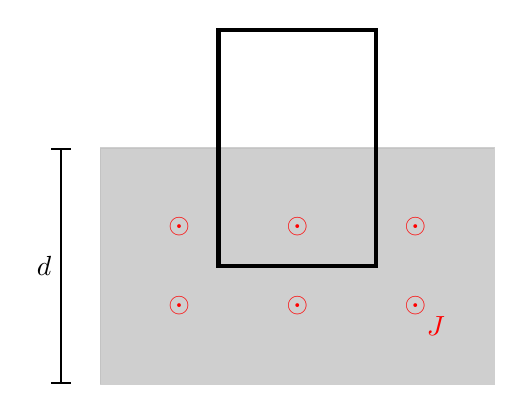
\begin{tikzpicture}
            \tikzstyle{current} = [color=red, ultra thick]
            \tikzstyle{conductor} = [color=lightgray, fill=lightgray, opacity=0.75]
            \tikzstyle{loop} = [ultra thick]
            \draw[conductor] (0, 0) rectangle (5, 3);
            %\draw (0, 0) grid (5, 3);
            \foreach \x in {1, 2.5, 4} {
                \foreach \y in {1, 2} {
                    \node[current] at (\x, \y) {\(\bm{\odot}\)};
                }   
            }
            \node[below right, current] at (4, 1) {\(\vv{J}\)};
            \draw[loop] (1.5, 1.5) rectangle (3.5, 4.5);
            \draw[thick, |-|] (-0.5, 0) -- (-0.5, 3);
            \node[left] at (-0.5, 1.5) {\(d\)};
        \end{tikzpicture}
        \caption{Finding the magnetic field inside a slab of current}
    \end{figure}
    If we want to know the magnetic field inside the slab then the set up for the Amp\'erian loop is similar but now one of the sides in the \(y\) direction should be inside the slab.
    We then use the field outside the loop that we already know to integrate along this loop.
    We find that
    \[B_{y,\text{in}} = -\mu_0Jz.\]
    \begin{figure}[ht]
        \centering
        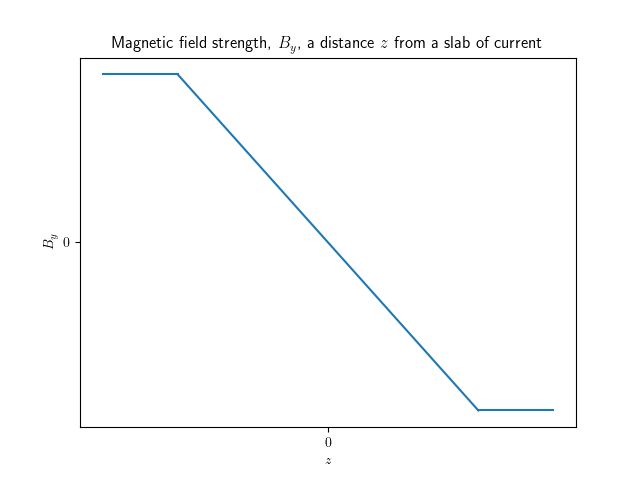
\includegraphics[scale=0.6]{magnetic_field_slab.png}
        \caption{The magnetic field strength, \(B_y\), a distance, \(z\), from a slab carrying current density, \(\vv{J}\).}
    \end{figure}

    \subsection{Toroid}
    A wire is curled up into a solenoid with \(n\) coils per unit length and radius \(R\).
    The solenoid is the curled up into a toroid of radius \(a > R\).
    \begin{figure}
        \centering
        \tikzsetnextfilename{toroid}
        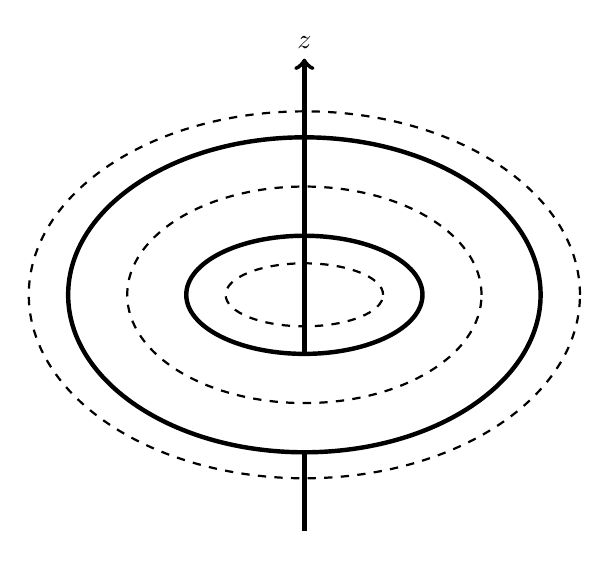
\begin{tikzpicture}
            \tikzstyle{axis} = [ultra thick]
            \tikzstyle{loop} = [thick, dashed]
            \tikzstyle{toroid} = [ultra thick]
            \draw[toroid] (0, 0) circle[x radius=3cm, y radius=2cm];
            \draw[toroid] (0, 0) circle[x radius=1.5cm, y radius=0.75cm];
            \draw[axis, ->] (0, -0.75) -- (0, 3);
            \draw[axis] (0, -2) -- (0, -3);
            \node[above] at (0, 3) {\(z\)};
            \draw[loop] (0, 0) circle[x radius=2.25cm, y radius=1.375cm];
            \draw[loop] (0, 0) circle[x radius=3.5cm, y radius=2.33cm];
            \draw[loop] (0, 0) circle[x radius=1cm, y radius=0.4cm];
        \end{tikzpicture}
        \caption{Finding the magnetic field inside a toroid}
        \label{fig:toroid}
    \end{figure}
    Figure~\ref{fig:toroid} shows a toroid (normal lines) with three possible Amp\'erian loops (dashed lines).
    The easiest loop to consider is the one that is entirely inside the hole of the toroid.
    Clearly there is no current enclosed in this so the magnetic field in the hole must be zero.
    Next we consider the outer most loop.
    At first it may seem like current does pass trough this but we must remember that the direction is important and therefore the \emph{net} current is zero as there is just as much current in both directions since the current is forming loops in the coil.
    Therefore outside of the toroid the magnetic field must be zero.
    The only Amp\'erian loop with a net current enclosed is the one that is in the toroid.
    
    All of the current element that pass through it are in the \((\rho, z)\)-plane, this means that \(\vv{B}\) can only be in the \(\ve{\varphi}\) direction.
    If the loop has radius \(\rho\) then we find that
    \[\oint_C\vv{B}\cdot\dd{\vv{l}} = 2\pi\rho B_\varphi = \mu_0I_\enc = \mu_0n2\pi aI\]
    where \(I\) is the current carried by the wire.
    Rearranging this we get
    \[B_\varphi = \frac{\mu_0nIa}{\rho}.\]
    
    \subsection{Magnetic Vector Potential}
    \begin{theorem}{}{}
        The following are equivalent for a vector field, \(\vv{B}\colon\reals^3 \to \reals^3\):
        \begin{enumerate}
            \item \(\div\vv{B} = 0\), in which case we call the field \define{solenoidal}.
            \item There exists a vector field, \(\vv{A}\colon\reals^3\to\reals^3\) such that \(\vv{B} = \curl\vv{A}\), in which case we call \(\vv{A}\) the \define{vector potential} of \(\vv{B}\).
            \item The surface integral
            \[\int_S\vv{B}\cdot\dd{\vv{S}}\]
            is independent of the shape of the surface, \(S\), for a given boundary curve.
            In particular
            \[\oint_S\vv{B}\cdot\dd{\vv{S}} = 0\]
            for any closed surface \(S\).
        \end{enumerate}
    \end{theorem}
    Maxwell's second equation tells us that \(\div\vv{B} = 0\) so there must exist \(\vv{A}\) such that
    \[\vv{B} = \curl\vv{A}.\]
    We call \(\vv{A}\) the \define{magnetic vector potential}.
    Compare this to the scalar electric potential, \(\varphi\) for a stationary electric field where we have
    \[\vv{E} = -\grad\varphi.\]
    
    \subsubsection{Poisson's Equation for the Vector Potential}
    Amp\`ere's law is
    \[\curl\vv{B} = \curl(\curl\vv{A}) = \mu_0\vv{J}.\]
    Applying a vector calculus identity we have
    \begin{equation}\label{eqn:curl A = laplacian A - grad div A = -mu0 J}
        -\curl(\curl\vv{A}) = \laplacian\vv{A} - \grad(\div\vv{A}) = -\mu_0\vv{J}.
    \end{equation}
    This is the most general form that we can find making no assumptions about the potential.
    However we have a \define{gauge freedom} that allows us to modify the potentials in a certain way without effecting the physics.
    That is the modified potentials given the same electric and magnetic fields.
    We have already seen this for the electric field.
    If we have two potentials, \(V(\vv{r})\) and \(\tilde{V}(\vv{r}) = V(\vv{r}) + C\) where \(C\in\reals\) then
    \[-\grad V(\vv{r}) = \vv{E}\]
    by definition but also
    \[-\grad\tilde{V} = -\grad(V + C) = -\grad V - \grad C = -\grad V = \vv{E}.\]
    Thus the field is unchanged by the addition of a constant to the potential.
    Similarly with the vector potential if we have two potentials, \(\vv{A}(\vv{r})\) and \(\vv{\tilde{A}}(\vv{r}) = \vv{A}(\vv{r}) + \grad\varphi(\vv{r})\) where \(\varphi\colon\reals^3\to\reals\) then
    \[\curl\vv{A} = \vv{B}\]
    by definition but also
    \[\curl\vv{\tilde{A}} = \curl(\vv{A} + \grad\varphi) = \curl\vv{A} + \curl\grad\vv{A} = \curl\vv{A} = \vv{B}.\]
    Thus the field is unchanged by the addition of a gradient field to the potential.
    
    We use this gauge freedom to select a gauge (a condition on the potential) that simplifies equations.
    One of the most common gauges to choose is the \define{Coulomb gauge}:
    \[\div\vv{A} = 0.\]
    For all magnetic fields, \(\vv{B}\), it is always possible to define a potential, \(\vv{A}\), such that
    \[\curl\vv{A} = \vv{B},\qquad\text{and}\qquad \div\vv{A} = 0.\]
    Given a potential \(\vv{A'}\) that satisfies the first of these condition then \(\vv{A} = \vv{A'} + \grad\varphi\) also satisfies the first condition.
    We can also require that
    \[\div\vv{A} = \div\vv{A'} + \div\grad\varphi = \div\vv{A} + \laplacian\varphi = 0 \implies \laplacian\varphi = -\div\vv{A}.\]
    This is simply \gls{pe} for \(\varphi\).
    We know that this has a solution
    \[\varphi(\vv{r}) = \frac{1}{4\pi}\int\frac{\div\vv{A}(\vv{r'})}{\abs{\vv{r} - \vv{r'}}^3}\dd[3]{r'}.\]
    
    In the Coulomb gauge equation~\ref{eqn:curl A = laplacian A - grad div A = -mu0 J} becomes
    \[\laplacian\vv{A} = -\mu_0\vv{J}.\]
    This is actually three equations, one for each component:
    \[\laplacian A_i - -\mu_0 J_i.\]
    So we have reduced equation~\ref{eqn:curl A = laplacian A - grad div A = -mu0 J} to \gls{pe} by carefully choosing a gauge.
    This means that we can use all of the methods we have already developed for \gls{pe}.
    In particular we have the explicit solution
    \[\vv{A}(\vv{r}) = \frac{\mu_0}{4\pi}\int\frac{\vv{J}(\vv{r'})}{\abs{\vv{r} - \vv{r'}}}\dd[3]{r'}.\]
    For example using this we can find that the magnetic dipole has a potential of
    \[\vv{A} = \frac{\,u_0}{4\pi}\frac{\vv{m}\times\vv{r}}{r^3}.\]
    
    \subsection{Summary of Statics}
    The electric field, \(\vv{E}\), and magnetic field, \(\vv{B}\), are defined such that for a charge, \(q\), moving at velocity \(\vv{v}\), the force on the charge is given by the Lorentz force law:
    \[\vv{F} = q(\vv{E} + \vv{v}\times\vv{B}).\]
    
    \subsubsection{Electrostatics}
    A static electric field is created by a stationary charge distribution, \(\rho\), meaning \(\partial_t\rho = 0\).
    The empirical law from which we derive everything else is Coulomb's law:
    \[\vv{F} = \frac{1}{4\pi\varepsilon_0}\frac{qQ}{r^2}.\]
    From this we can derive Maxwell's first and third laws, which are
    \[\div\vv{E} = \frac{\rho}{\varepsilon_0} \iff \oint_S\vv{E}\cdot\dd{\vv{S}} = \frac{Q_\enc}{\varepsilon_0},\tag{MI}\]
    and
    \[\curl\vv{E} = \vv{0} \iff \oint_C\vv{E}\cdot\dd{\vv{l}} = 0.\tag{MIII static}\]
    This last equation allows us to define an electrostatic potential, \(V\), such that
    \[\vv{E} = -\grad V.\]
    Combining this with Maxwell's first equation we get \gls{pe}:
    \[\laplacian V = -\frac{\rho}{\varepsilon}.\]
    
    \subsubsection{Magnetostatics}
    A static magnetic field is created by a steady current density, \(\vv{J}\), meaning \(\partial_t\vv{J} = \vv{0}\).
    The empirical law from which we derive everything else is the Biot Savart law:
    \[\dd{\vv{B}}(\vv{r}) = \frac{\mu_0}{4\pi}\frac{\dd{\vv{\current}}(\vv{r'})\times(\vv{r} - \vv{r'})}{\abs{\vv{r} - \vv{r'}}^3}.\]
    From this we can derive Maxwell's second and fourth laws, which are
    \[\div\vv{B} = 0 \iff \oint_S\vv{B}\cdot\dd{\vv{S}} = 0,\tag{MII}\]
    and
    \[\curl\vv{B} = \mu_0\vv{J} \iff \oint_C\vv{B}\cdot\dd{l} = \mu_0\int_S\vv{J}\cdot\dd{\vv{S}}.\tag{MIV static}\]
    The first of these allows us to define a vector potential, \(\vv{A}\), such that
    \[\vv{B} = \curl\vv{A}.\]
    Combining both of these equations, and working in the Coulomb gauge, \(\div\vv{A} = 0\), we get \gls{pe}:
    \[\laplacian\vv{A} = -\mu_0\vv{J}.\]